\chapter{Development}

\section{Game design}
This section describes the design of \textit{Micorrizas}, presenting the main elements that define the game and support its educational objectives. Specifically, it introduces the game concept, narrative, gameplay loop, game scenes, mechanics, and the principal design decisions adopted during the development process.

\subsection{Game concept}

\textit{Micorrizas} is a multiplayer (2-6) cooperative location-based game in which players move through real-world locations shown on a map, triggering quests that consist of short collaborative challenges with varied mechanics.

\textit{Micorrizas} is based on the educational activity carried out in the \textit{Jardín de los Sentidos} as part of the subject related to the natural environment in Early Childhood Education. In this activity, students separated in groups visit the garden and work directly with the natural space through observation, identification and interpretation tasks. The aim is for students to understand the educational potential of nearby natural environments and to learn about the biodiversity of the garden through direct interaction with plants, sensory areas and ecological elements.

Since the original activity takes place outdoors and requires students to move through the different areas of the garden, \textit{Micorrizas} was designed as a mobile and geolocated experience. The mobile device makes it possible to guide the students through the physical space, detect their position and activate missions when the group reaches specific areas. In this way, the game preserves the relationship with the real environment while adding a digital layer of interaction, narrative progression and feedback.

The content of the game is organised through missions linked to the senses represented in the garden (see Figure \ref{fig:jardin}). Each quest focuses on a specific type of perception or knowledge: visual recognition of plants, identification of sounds, deduction of species from tactile characteristics, the relationship between fruits and species, and classification of plants according to their uses. The design of each quest was defined by combining the educational purpose of the original activity by each area of the garden (i.e., Garden of Sight, Garden of Hearing, Garden of Touch, Garden of Taste, Garden of Smell) with interaction models suitable for mobile devices. This type of interaction is detailed in Section \ref{sec:mechanics}.

\begin{figure}[H]
    \centering
    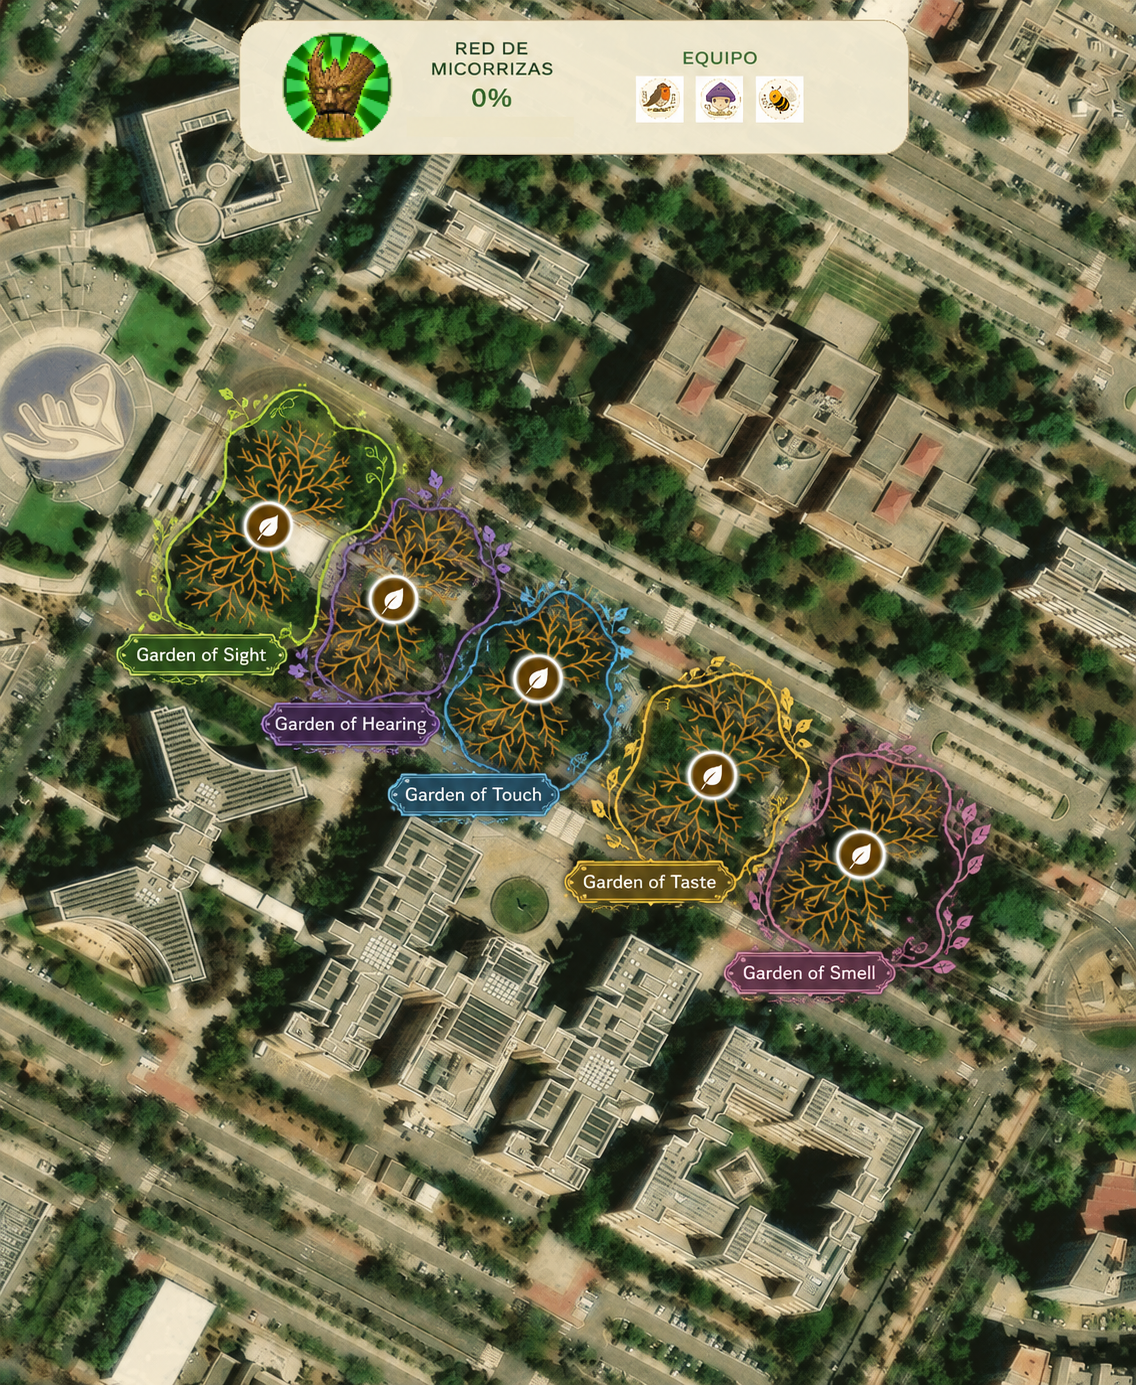
\includegraphics[width=0.6\textwidth]{img/MapaNombres.png}
    \caption{The \textit{Jardín de los Sentidos}, organised into its sensory zones}
    \label{fig:jardin}
\end{figure}

Cooperation plays a central role in the design. Quests are completed as a group and the score obtained belongs to all members in the same game. Some quests rely on discussion and collective memory, while others distribute information across devices to encourage communication between players. This cooperative gameplay makes collaboration an active part of how the game functions and reflects the social nature of the original learning activity.

Main character’s narrative and the mycorrhizal network give unity to the experience. Each mission represents the recovery of a part of the garden and contributes to rebuilding the lost connection between the sensory zones. The game’s progression is presented as a symbolic restoration of the natural environment, linking players’ actions to the observation, interpretation and care of biodiversity.

% Imagen del mapa zonas definidas







\subsection{Lore}
Deeproot (see Figure \ref{fig:Deeproot}) is the main character in \textit{Micorrizas}  and acts as the game’s narrative guide. He is an Ent, a creature directly linked to the flora of the \textit{Jardín de los Sentidos}, whose role is to protect and manage the area’s natural resources. Due to the slowness inherent to his species and the progressive deterioration of the garden, Deeproot seeks the help of a group of adventurers, represented by the players, to restore the lost balance.
\begin{figure}[htpb]
    \centering
    
\includegraphics[width=0.3\textwidth]{img/Deeproot.png}
    \caption{Deeproot the main character}
    \label{fig:Deeproot}
\end{figure}

The story begins with a conflict caused by the negligence of the human race. For a long time, natural spaces and their biodiversity have been polluted, ignored and displaced, weakening the relationship between people and the environment. In the past, nature flourished throughout the university’s grounds, and the \textit{Jardín de los Sentidos} occupied a central place within that ecosystem. It was the heart of all the flora in the realm and maintained a connection with the rest of the green spaces via an underground network formed by conduits covering the plants’ roots, as can be seen in Figure \ref{fig:mycorrhizae}.

\vspace{0.5cm}
\begin{figure}[H]
    \centering
    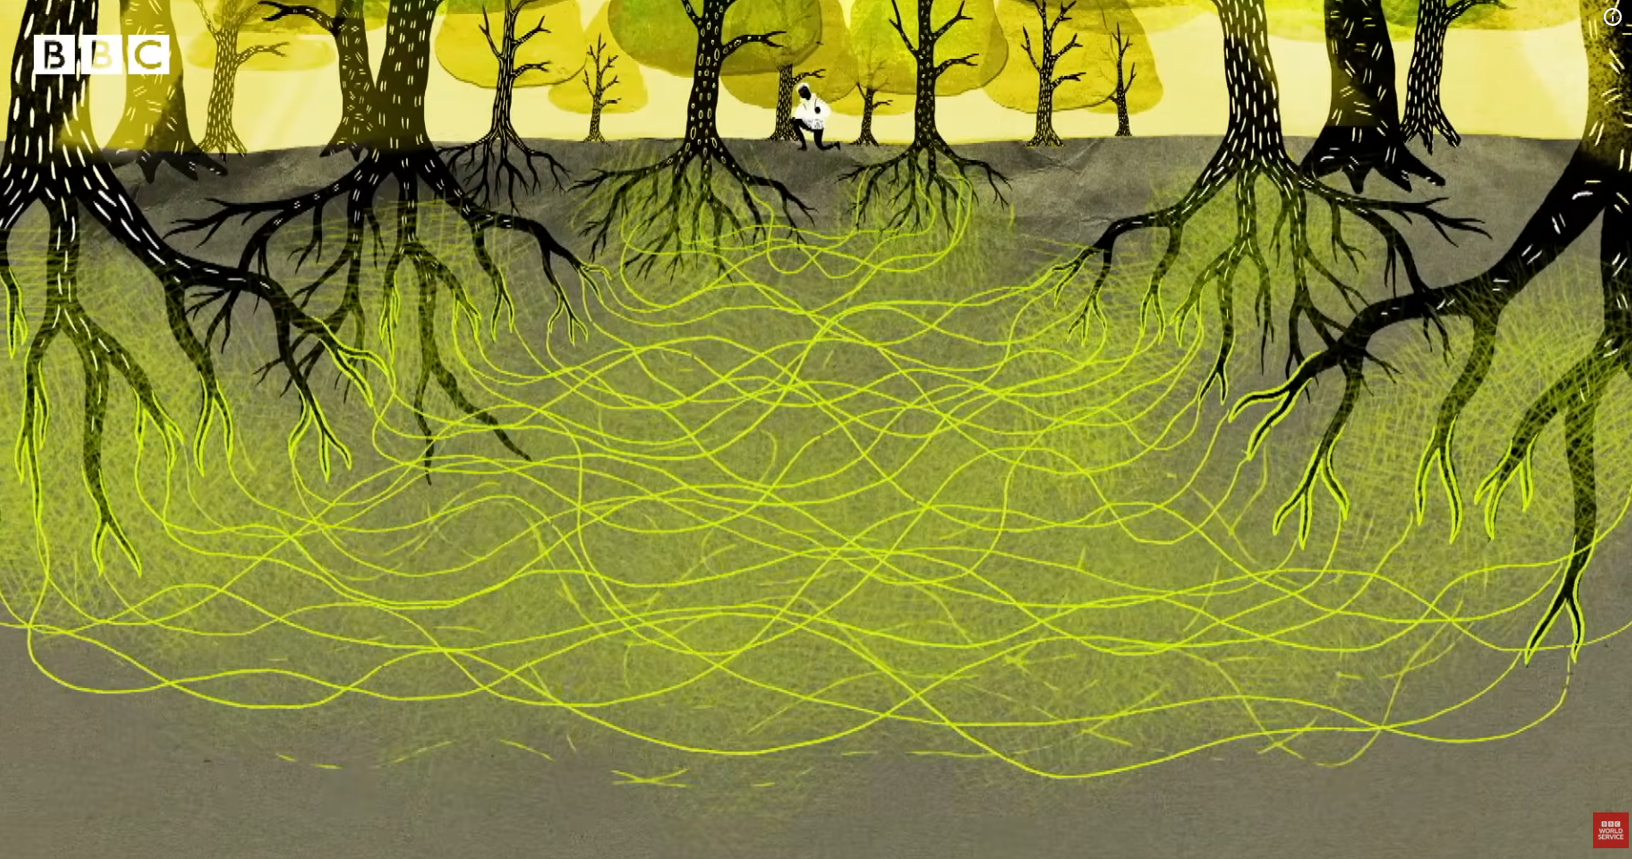
\includegraphics[width=\textwidth]{img/Micorrizas.png}
    \caption{Mycorrhizae by BBC World Service\protect\footnotemark}
    \label{fig:mycorrhizae}
\end{figure}

\footnotetext{Resource: BBC World Service \cite{BBCWorldService}.}

These conduits were made up of mycorrhizae, the symbiotic relationship between a fungus’s mycelium and a plant’s roots, and enabled the \textit{Jardín de los Sentidos} to send nutrients, signals and information to the rest of the flora. Thanks to this network, the plants were able to remain connected, and the garden functioned as a living organism capable of perceiving, remembering and transmitting knowledge through its senses.

At present, this network is fragmented and weakened. The garden’s senses have lost part of their memory, and Deeproot can no longer transmit information correctly via the mycorrhizae. Even so, the network can still be restored. To achieve this, players must explore the \textit{Jardín de los Sentidos}, complete the various missions associated with each sensory zone, and help restore the lost connections.

Once the group has managed to restore the garden’s senses, Deeproot will once again be able to channel information through the mycorrhizal network. The restoration of this connection symbolises the recovery of the bond between humans and the natural environment, as well as the ability to observe, understand and appreciate the biodiversity that forms part of the garden.


\subsection{Game Loop}
The game loop in \textit{Micorrizas} is structured around the physical exploration of the \textit{Jardín de los Sentidos} and the triggering of quests via geolocation. As Figure \ref{fig:gameloop} shows, the experience begins on the connection screen, where one player creates the game as the host and the other participants join using a code. Once the session has been established, all players access the map scene, which serves as the central hub for navigation and group coordination.

Upon entering the map scene, the system checks the players’ positions. If the group is outside the \textit{Jardín de los Sentidos}, Deeproot appears to indicate that assistance can only begin once everyone has arrived at the garden. This initial condition links the start of the game to physical presence in the space and reinforces the geolocation-based nature of the experience.

Once all players are within the playable area, Deeproot introduces the main objective: to explore the garden and find the missions needed to repair the mycorrhizal network. From this point onwards, the group can move freely around the map. Progression follows a non-linear structure, as the five missions associated with the senses can be completed in any order. This decision allows the journey to adapt to the group’s actual movement through the garden and avoids imposing a rigid sequence on the physical space.

The main loop is repeated in each sensory zone. Players explore the environment, enter a mission’s activation area, receive the corresponding narrative context, solve the mission cooperatively, and receive feedback on their result. Upon completing the mission, the system records the group’s score, marks that zone as completed, and returns the group to the map to continue their exploration. The group of adventurers can only complete each mission once. However, they can replay the entire game to achieve a higher score, as if they score less than 5, they will not have succeeded in restoring the mycorrhizal network.
\begin{figure}[H]
    \centering
    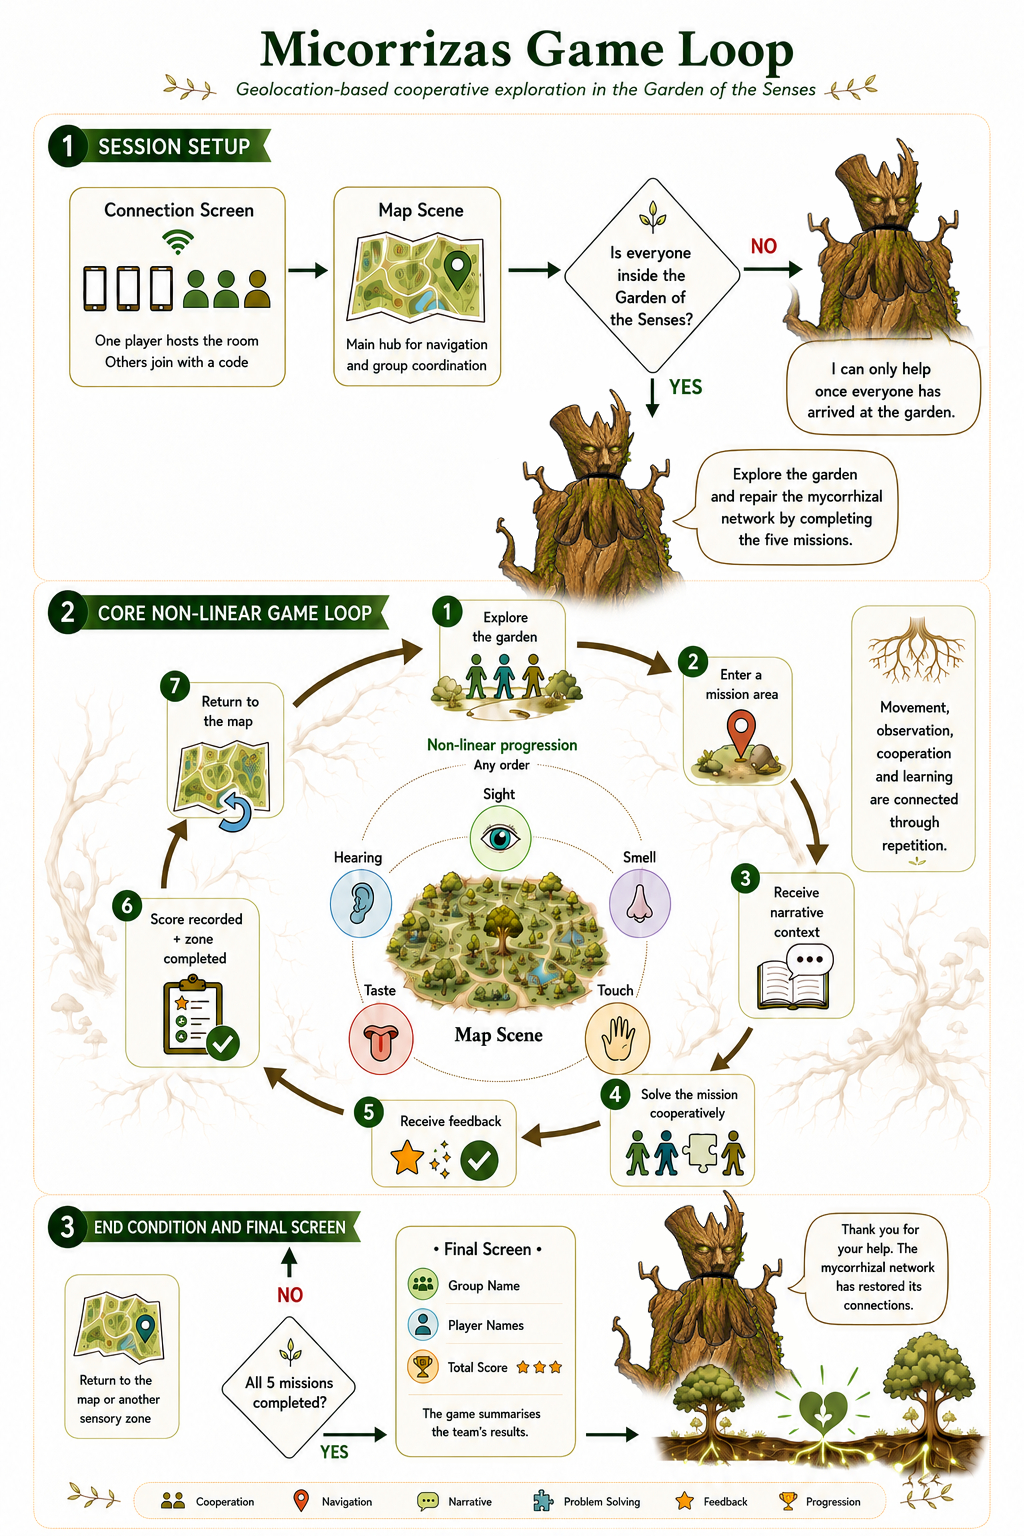
\includegraphics[width=0.9\textwidth]{img/MicorrizasGameLoop.jpg}
    \caption{Micorrizas game loop}
    \label{fig:gameloop}
\end{figure}
Once all five missions have been completed, the game proceeds to the final screen. This scene displays the group’s name, the participants’ names and the group score achieved during the session. Deeproot concludes the experience by thanking the players for their help and explaining that the mycorrhizal network has restored its connections. This conclusion serves a dual purpose: it summarises the team’s results and provides a narrative conclusion to the journey through the garden. These results can then be used by the course lecturers to mark the activity on which the project is based.




\subsection{Scenes from the game}

The \textit{Micorrizas} experience is organised into several scenes, each one associated with a specific function within the overall structure of the game. These scenes separate the main stages of the experience: creating or joining a cooperative session, exploring the garden, completing the sensory missions, and presenting the final result.

\textbf{Lobby system scene:} This scene is used to start the game and create the cooperative session. One player acts as host and generates a game code (see Figure \ref{fig:lobbyScene}), while the remaining players use that code to join the same session. Its main purpose is to ensure that all participants are connected before the shared experience begins.

\begin{figure}[H]
    \begin{multicols}{2} % Inicio de las dos columnas
        \begin{center}
            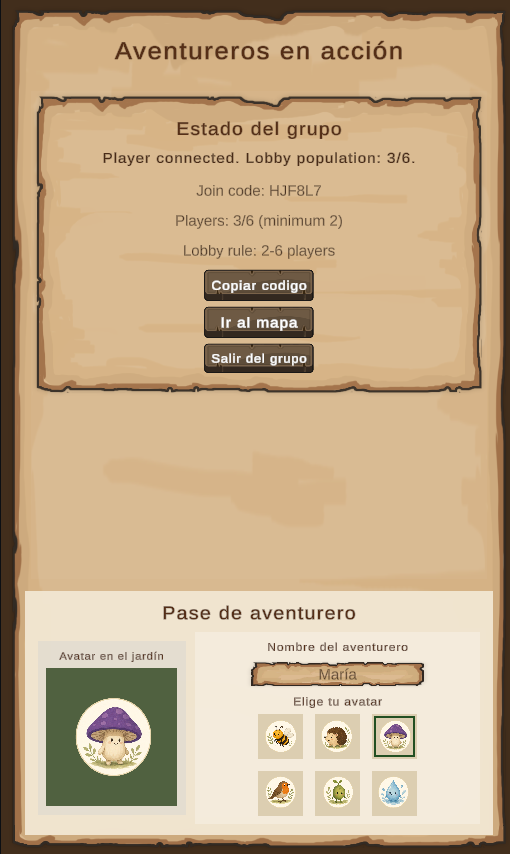
\includegraphics[width=0.4\textwidth]{img/ingame/Lobby.png}
            \caption{Lobby scene in game}
            \label{fig:lobbyScene}
        \end{center}
        
        \columnbreak
        
        \begin{center}
            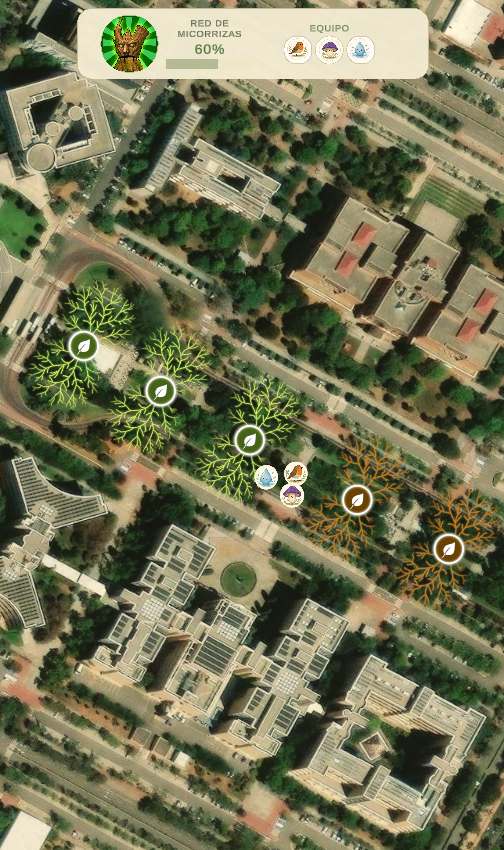
\includegraphics[width=0.4\textwidth]{img/ingame/mapInGame.png}
            \caption{Map scene in game}
            \label{fig:mapInGame}
        \end{center}
    \end{multicols} % Fin de las dos columnas
\end{figure}

\textbf{Map scene:} This is the main navigation screen of the game (see Figure \ref{fig:mapInGame}). It represents the \textit{Jardín de los Sentidos} using ArcGIS and displays the position of the players within the physical space. From this scene, the system detects the sensory zones, activates the corresponding missions and shows the group which areas have already been completed.

\textbf{Quest scenes:} These scenes contain the main playable activities. They share a common interface structure, with a header that presents the mission objective, the relevant score or progress, and the instructions needed to complete the activity. Each mission is completed cooperatively, and the result obtained is shared by all members of the same session. At the end of each mission, the group receives a score between 0 and 10, which contributes to the overall progress of the game.

\textbf{Garden of Sight mission:} In this scene,  plant species images and the corresponding scientific names are shown using cards.

\textbf{Garden of Hearing mission:} The scene presents an interface centred on an audio player together with a distorted black-and-white image that provides a visual clue related to the sound being played.

\textbf{Garden of Touch mission:} The scene displays a sequence of textual clues describing the physical and sensory characteristics of a plant, together with the interface elements required to submit the group's answer.

\textbf{Garden of Taste mission:} The scene contains a set of face-down cards arranged in a grid, displaying illustrations of plants and fruits that are revealed as the activity progresses.

\textbf{Garden of Smell mission:} The scene presents a collection of plant illustrations together with several labelled category areas, allowing players to organise the elements within the interface.

\textbf{Final result scene:} This scene presents the conclusion of the experience after the five main missions have been completed. It displays the group name, the names of the participants and the final score achieved. Deeproot also appears again to close the narrative and thank the players for helping to restore the mycorrhizal network.


\newpage
\subsection{Game Mechanics}
\label{sec:mechanics}
The game mechanics of \textit{Micorrizas} are organised into two levels: a core mechanic common to the entire experience, and a set of specific game mechanics associated with each mission. 

The core game mechanic is the physical exploration of the \textit{Jardín de los Sentidos}. Players advance by moving through the real space, and the system uses geolocation to detect when the group enters a sensory zone. When everyone has been in that area for 5 seconds, the corresponding mission is triggered and the player’s action shifts from the map to the quest scene. Figure \ref{fig:triggers} shows the area corresponding to each zone.

\begin{figure}[H]
    \centering
    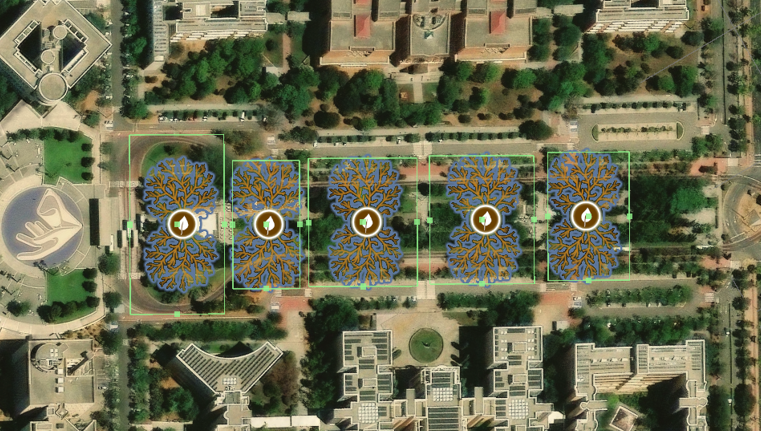
\includegraphics[width=\textwidth]{img/Triggers.png}
    \caption{Triggers of the garden}
    \label{fig:triggers}
\end{figure}

This main game mechanic allows movement through the garden to form part of the gameplay itself. Players use the map to orient themselves, locate pending zones and check the group’s progress. Geolocation links the participants’ real-world position to the narrative and gameplay progression, so that each mission is tied to a specific location within the environment.

The specific game mechanics associated with each mission are described below.

\newpage
\textbf{Garden of Sight}
\newline
In the Garden of Sight, the mission uses a card-swiping mechanic (see Figure \ref{fig:quest1}). In each round, a card appears showing an image of a plant and its scientific name. Players must decide whether that species has been observed in the Garden of Sight. To answer, they swipe the card to the right if they believe it belongs in that area, and to the left if they believe it does not. This interaction is well suited to mobile devices because it is quick, straightforward and easy to understand. The mission develops visual discrimination, as players must compare the information on the card with what they are observing in the real environment.


\begin{figure}[H]
    \centering
    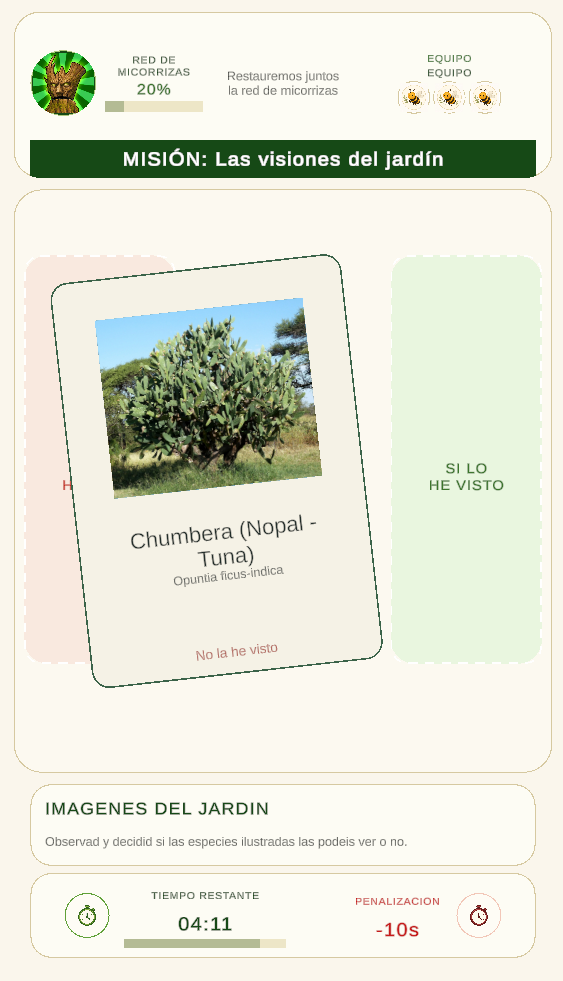
\includegraphics[width=0.4\textwidth]{img/ingame/quest1noVisto.png}
    \caption{Quest in the Garden of Sight with card-swiping mechanic}
    \label{fig:quest1}
\end{figure}

\newpage
\textbf{Garden of Hearing}
\newline
In the Garden of Hearing, the mission combines sound identification and cross-device cooperation. One player plays an audio clip related to the garden and the other devices display possible answers (see Figure \ref{fig:quest2-1} and \ref{fig:quest2-2}). The correct answer appears on only one of the mobiles, so the group must communicate to locate and select it. The mechanics draw on exercises involving the association of sound and word, alongside a distribution of answers among participants to reinforce collaboration. After each round, the device responsible for the audio changes, allowing different players to take on different roles during the mission.

\begin{figure}[H]
    \begin{multicols}{2} % Inicio de las dos columnas
        \begin{center}
            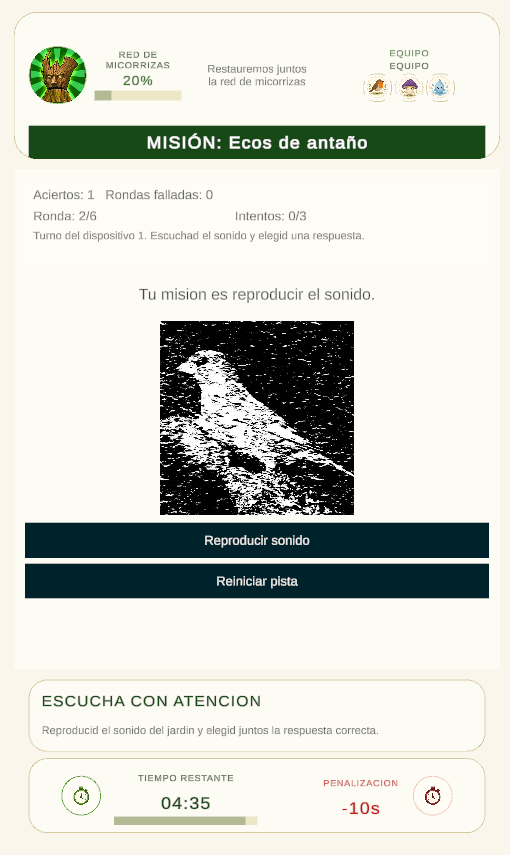
\includegraphics[width=0.4\textwidth]{img/ingame/quest2audio.png}
            \caption{Point of view of the player playing the audio}
            \label{fig:quest2-1}
        \end{center}
        
        \columnbreak
        
        \begin{center}
            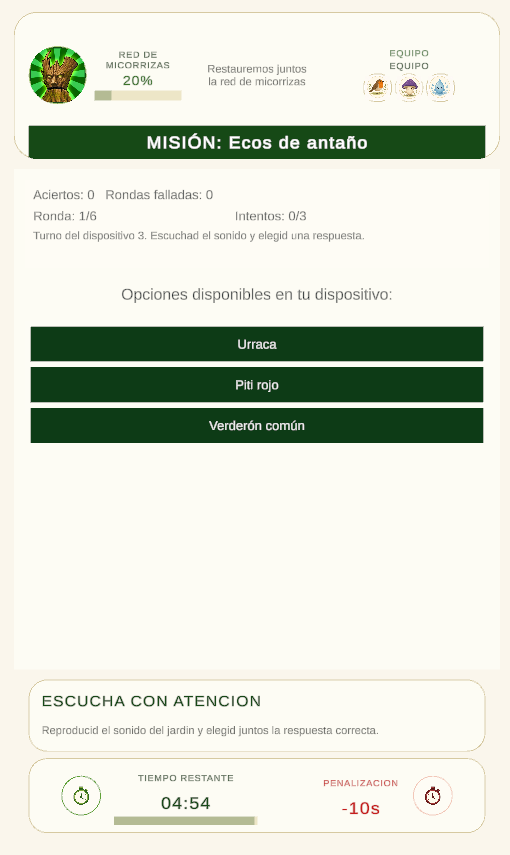
\includegraphics[width=0.4\textwidth]{img/ingame/quest2choices.png}
            \caption{Point of view of the player with answers}
            \label{fig:quest2-2}
        \end{center}
    \end{multicols} % Fin de las dos columnas
\end{figure}

\newpage
\textbf{Garden of Touch}
\newline
In the Garden of Touch, the mission is based on a progressive deduction mechanic. Players must write the name of a plant that might be found in that area of the garden. Each attempt reveals certain information. Initially, the system reveals general characteristics, such as roughness or shape. As new attempts are made, more specific clues are unlocked, such as characteristics of the fruit or type of plant. Furthermore, all these characteristics have a background colour: green if that information matches the plant in question, orange if it is similar, and red if it is completely unrelated (see Figure \ref{fig:quest3}).

\begin{figure}[H]
    \centering
    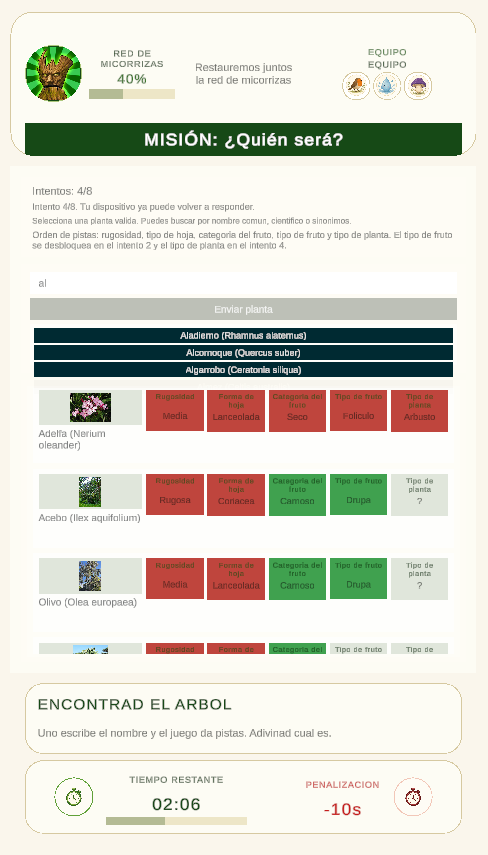
\includegraphics[width=0.4\textwidth]{img/ingame/quest3.png}
    \caption{Quest in the Garden of Touch,  trying to guess what kind of plant it is}
    \label{fig:quest3}
\end{figure}

\newpage
\textbf{Garden of Taste}
\newline
In the Garden of Taste, the mission uses a memory-matching mechanic (Figure \ref{fig:quest4-3} and \ref{fig:quest4-2}). Each device displays several face-down cards relating to fruits or plants in the garden. Players can reveal cards on their own devices, but pairs are never complete on a single mobile. To solve the mission, the group must communicate which cards each participant has discovered and coordinate to find the correct matches.

\begin{figure}[H]
    \begin{multicols}{2} % Inicio de las dos columnas
        \begin{center}
            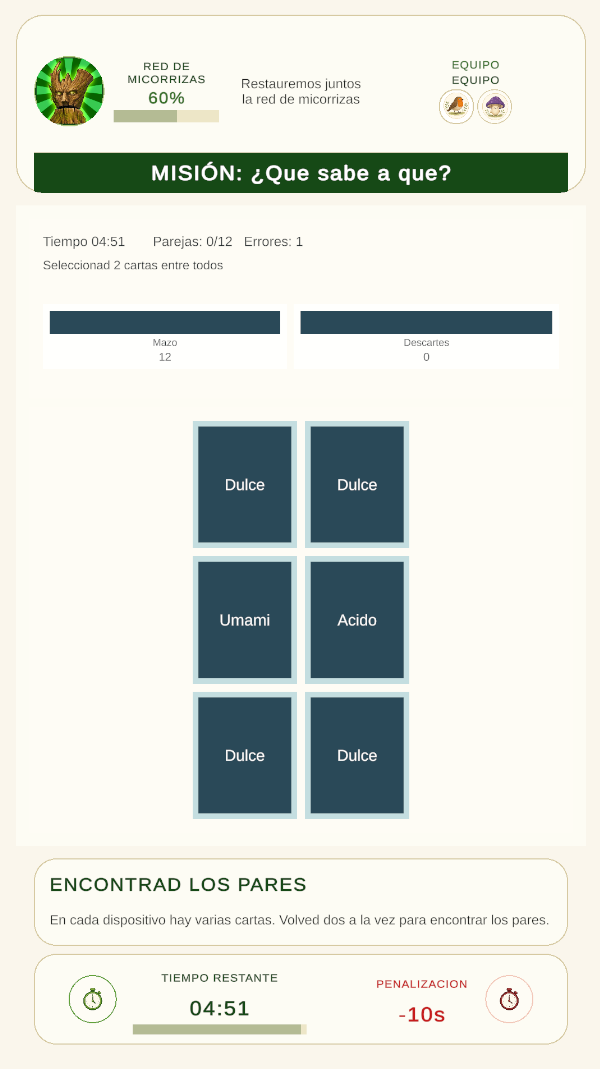
\includegraphics[width=0.4\textwidth]{img/ingame/quest4-3.png}
            \caption{Quest in the Garden of Taste with cards face down}
            \label{fig:quest4-3}
        \end{center}
        
        \columnbreak
        
        \begin{center}
            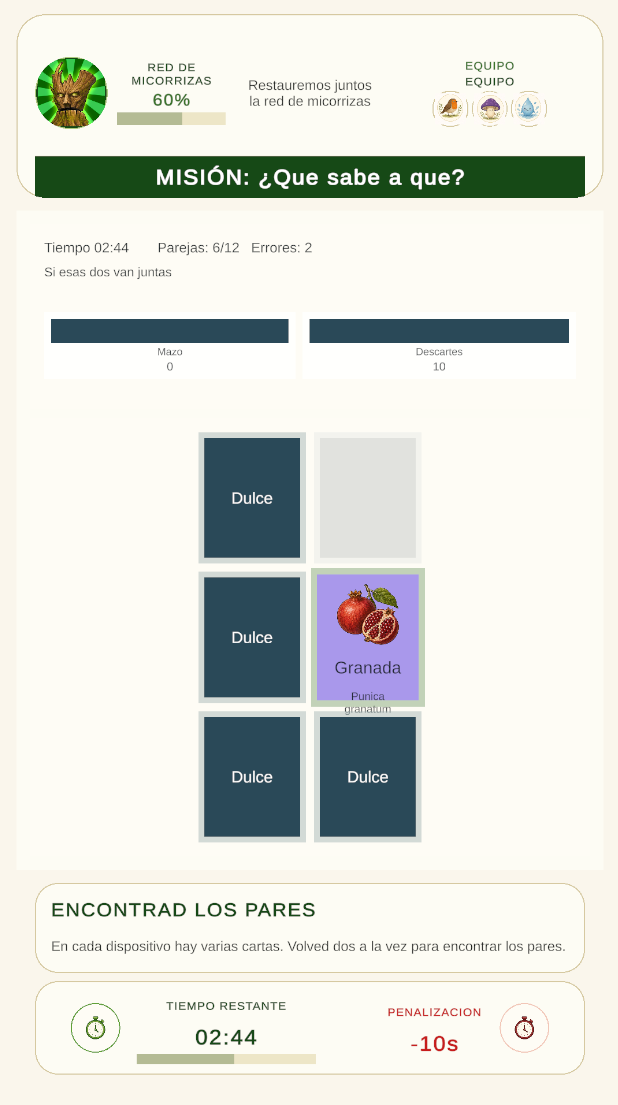
\includegraphics[width=0.4\textwidth]{img/ingame/quest4-2.png}
            \caption{Quest in the Garden of Taste unsing a memory-matching mechanic}
            \label{fig:quest4-2}
        \end{center}
    \end{multicols} % Fin de las dos columnas
\end{figure}

\newpage
\textbf{Garden of Smell}
\newline
In the Garden of Smell, the mission uses a drag-and-drop mechanic. Players are given cards bearing their own image and name, and must sort them into categories based on their use or function, such as decorative, culinary or medicinal. The interaction involves dragging each card to the corresponding section.

All quests share certain common elements. Firstly, there is cooperation, as challenges are solved as a group; this leads to shared progress, which tracks the areas completed and, in turn, results in a group score that applies to all players in the same room. Then there is the interface and the feedback system. The interface features the same elements: a top bar and a bottom bar. The feedback system uses a shaking animation and colours; as well as deducting points from our group of adventurers, it also subtracts 10 seconds from the time they have to complete each quest. These elements ensure that the game maintains its consistency, even though each quest uses a different form of interaction.

\subsection{Design decisions due to pedagogical objectives}
%TODO ESTO MEJOR AÑADIR UNA SUBSECCIÓN DESPUÉS DE MECHANICS (CREO) QUE SEA DESIGN DECISION DUE TO PEDAGOGIAL AIM (HAY QUE DARLE UNA VUELTA) Y PONER TODO ESTO PORQUE NO LLEGA A SER GAME CONCEPT SOLO, SÍ DECISIONES DE DISEÑO PERO TENIENDO EN CUENTA QUE ANTES HAS EXPLICADO LAS MECÁNICAS

The design of each quest was defined by combining the educational purpose of the original activity with interaction models suitable for mobile devices. Although each quest focuses on a different sensory experience, all of them were designed to encourage observation, discussion and collaboration, maintaining simple interactions appropriate for any user, regardless of their level of familiarity with technology.

The Garden of Sight quest is based on a swipe interaction. When a plant card appears on screen, players slide it to the right if they consider that the species has been observed in the Sight area, and to the left if they consider that it does not belong to that area. After each decision, the system provides feedback and updates the group score.

This interaction is simple, fast and well suited to mobile play. The binary gesture reduces interface complexity and allows players to focus on the recognition task. Since only one stimulus is presented at a time, the player’s attention remains centred on the plant profile and on the comparison with the real garden.

From a pedagogical perspective, the quest reinforces visual discrimination by requiring players to compare visual evidence, recall their observations during the route and make informed decisions. Immediate feedback helps them identify mistakes and progressively improve their understanding of the plants found in the garden.

Unlike the Sight quest, which relies primarily on visual recognition, the Sound mission focuses on auditory perception and communication between players. Its structure was inspired by two types of activities: audio-based association exercises, such as Duolingo \cite{duolingo} (see Figure \ref{fig:duo}), and collaborative answer distribution, similar to the dynamic used in Quizlet Live \cite{quizlet_live} (see Figure \ref{fig:quizlet0} and \ref{fig:quizlet1}). In each round, one device plays an audio clue related to a sound found in the garden, while the rest of the devices display different possible answers.

Only one of the devices contains the correct answer, requiring players to communicate, compare the available options and decide collectively which response should be selected. Once the answer has been submitted, the roles rotate so that every participant alternates between listening to the audio clue and providing possible answers. This design distributes responsibility across the group and encourages active participation throughout the activity. Educationally, the mission develops sound recognition and association, as well as strengthening communication and collaborative decision-making.

If you fail to choose an answer, the option will be disabled, the distorted image will be revealed a little more, as shown in these Figures \ref{fig:g0}, \ref{fig:g1}, \ref{fig:g2} and \ref{fig:g3}, and 10 seconds will be deducted from the time you have to complete that quest.

\begin{figure}[h]
    \begin{multicols}{2} % Inicio de las dos columnas
        \begin{center}
            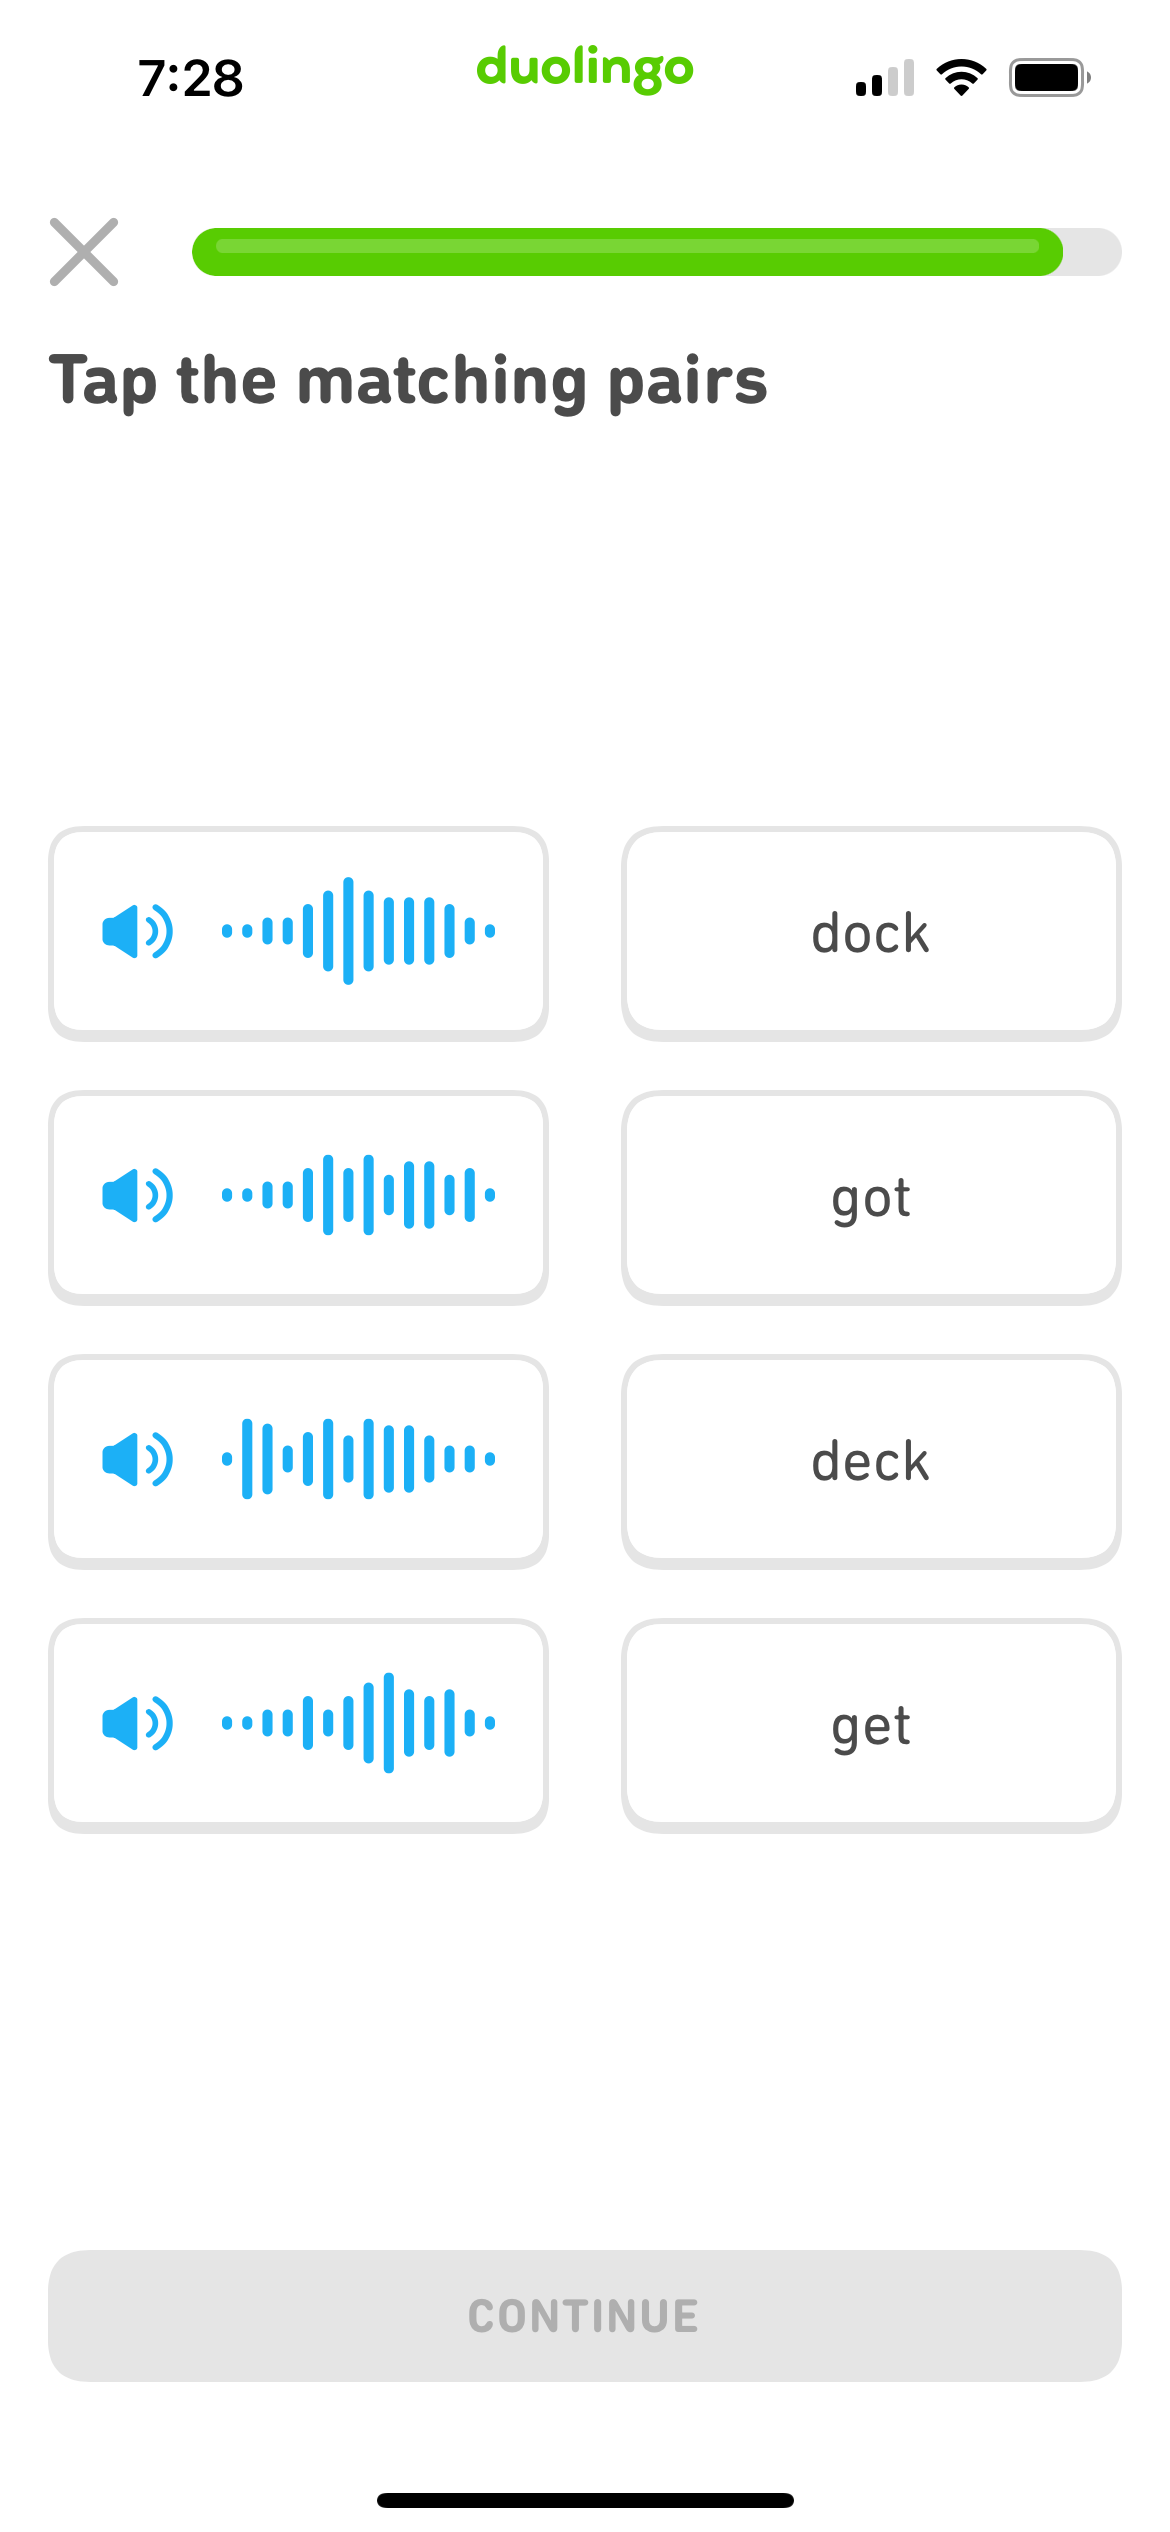
\includegraphics[width=0.3\textwidth]{img/Duolingo.png}
            \caption{An example of how Duolingo works}
            \label{fig:duo}
        \end{center}
        
        \columnbreak
        
        \begin{center}
            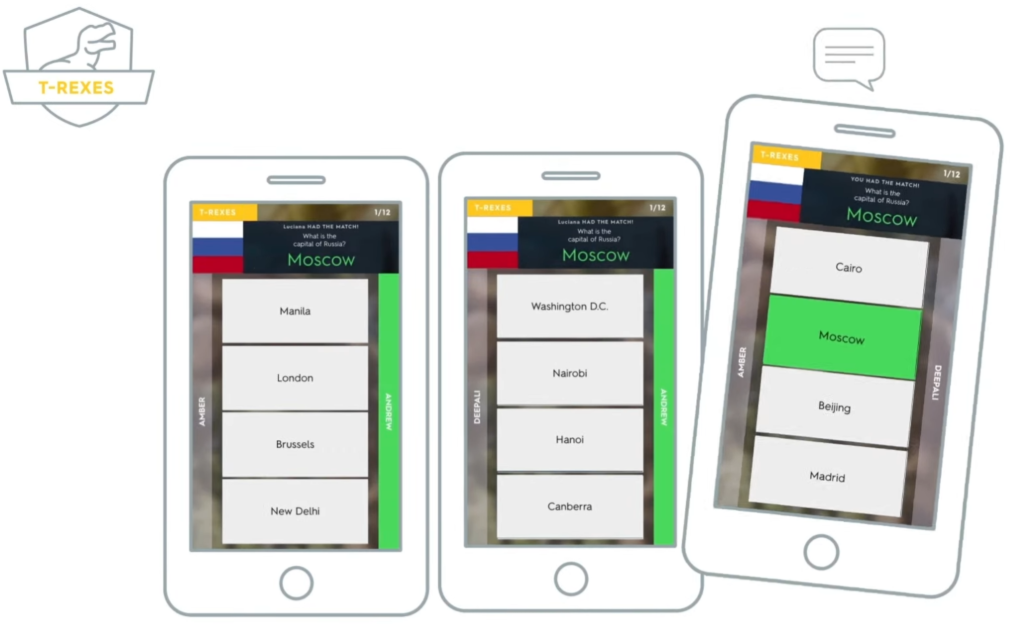
\includegraphics[width=0.5\textwidth]{img/QuizletLive1.png}
            \caption{An example of how Quizlet Live works}
            \label{fig:quizlet0}
        \end{center}
    \end{multicols} % Fin de las dos columnas
\end{figure}
\begin{figure}[H]
    \centering
    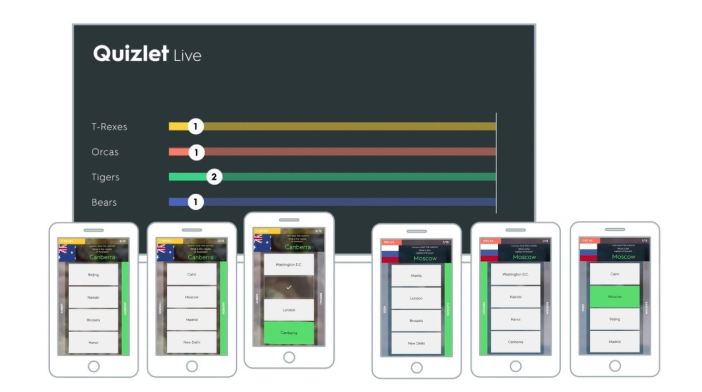
\includegraphics[width=0.6\textwidth]{img/QuizletLive0.png}
    \caption{Another example of how Quizlet Live works}
    \label{fig:quizlet1}
\end{figure}

\begin{figure}[h]
    \begin{multicols}{2} % Inicio de las dos columnas
        \begin{center}
            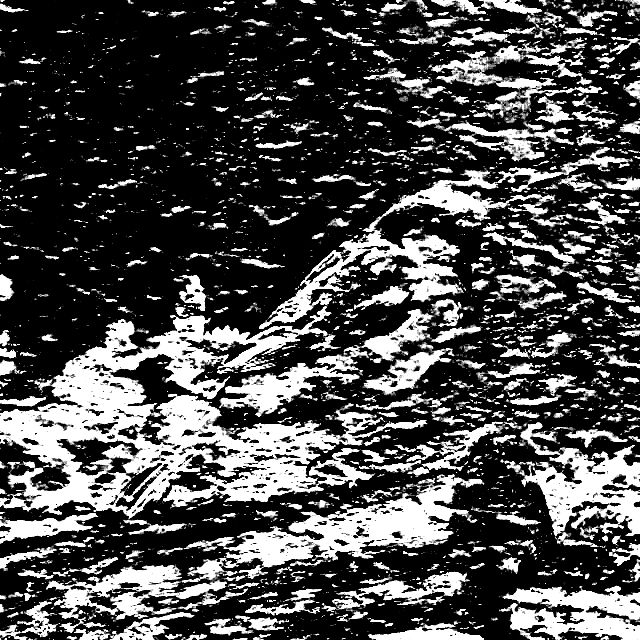
\includegraphics[width=0.3\textwidth]{img/Art/Gorrion0.jpg}
            \caption{The clue for the quest in the Garden of Hearing: opening image}
            \label{fig:g0}
        \end{center}
        
        \columnbreak
        
        \begin{center}
            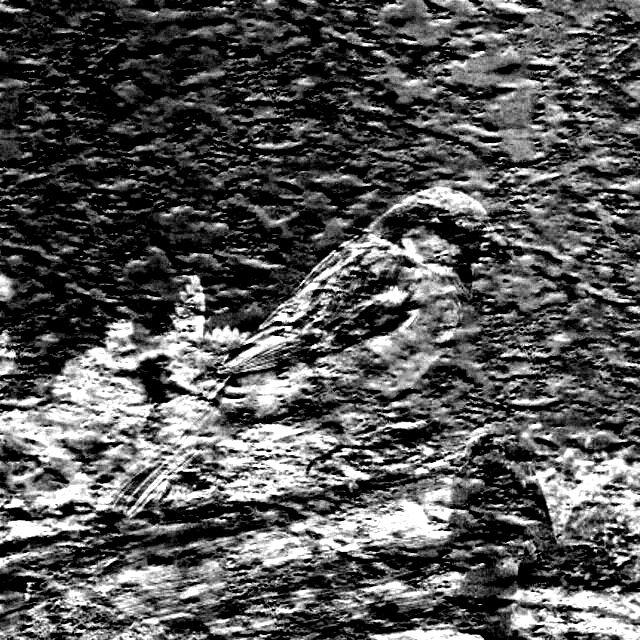
\includegraphics[width=0.3\textwidth]{img/Art/Gorrion1.jpg}
            \caption{The clue for the quest in the Garden of Hearing: next step a clearer image}
            \label{fig:g1}
        \end{center}
    \end{multicols} % Fin de las dos columnas
\end{figure}
\begin{figure}[h]
    \begin{multicols}{2} % Inicio de las dos columnas
        \begin{center}
            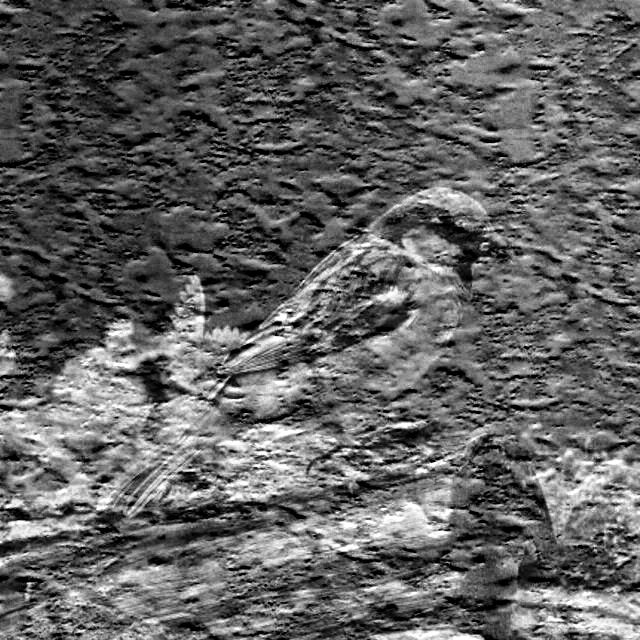
\includegraphics[width=0.3\textwidth]{img/Art/Gorrion2.jpg}
            \caption{The clue for the quest in the Garden of Hearing: next step, the image with the minimum filter}
            \label{fig:g2}
        \end{center}
        
        \columnbreak
        
        \begin{center}
            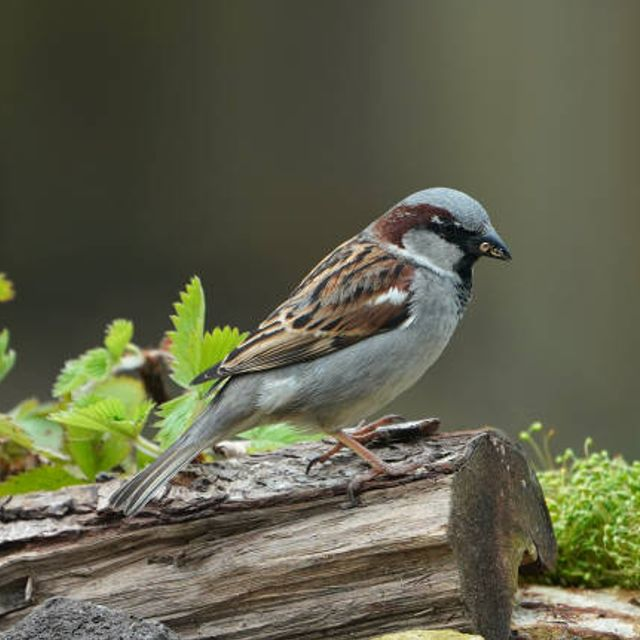
\includegraphics[width=0.3\textwidth]{img/Art/Gorrion3.jpg}
            \caption{The image shown as a solution}
            \label{fig:g3}
        \end{center}
    \end{multicols} % Fin de las dos columnas
\end{figure}



The mission of the Garden of Touch follows a different approach by presenting players with progressively more specific clues describing the physical and sensory characteristics of a plant. Rather than relying on immediate recognition, the mechanic encourages participants to discuss possible alternatives, compare their observations and gradually eliminate incorrect options before reaching a collective decision. This progression promotes critical thinking and maintains the interaction straightforward and easy to understand.

Similarly, the mission of the Garden of Taste adapts the traditional memory-card game into a cooperative experience. Instead of each player having access to all the information, cards are distributed across multiple devices, requiring participants to communicate the positions and contents they have discovered in order to complete the pairs successfully. As a result, a familiar mechanic becomes an activity that promotes teamwork, shared memory and information exchange.

Finally, the mission of the Garden of Smell requires players to classify different plant species according to categories such as decorative, culinary or medicinal uses. The drag-and-drop interaction provides an intuitive way of organising the information and keeps the information and keeping the interface clear an easy to navigate. From an educational perspective, this mechanic reinforces the relationship between plant species and their practical applications, encouraging players to discuss and justify each classification before reaching a common answer.

\subsection{Game art}
The visual design of \textit{Micorrizas} was created to support the educational and environmental tone of the project. Since the game takes place in the \textit{Jardín de los Sentidos} and focuses on biodiversity, the art direction follows a natural and friendly aesthetic. The predominant colour is green, which evokes vegetation, nature and ecological restoration. This is complemented by brown and earthy tones, especially in elements related to Deeproot, trees, roots and the mycorrhizal network.

The game combines two visual approaches. The map has a realistic function, as it represents the physical space where the players move. Its purpose is to help players understand their position in the garden and connect the digital experience with the real environment. In contrast, the character, interface elements and icons use a simpler and cleaner style, based on flat colours, clear shapes and readable visual elements. This contrast allows the map to preserve its connection with the real location and keeps the interface accessible on a mobile screen.

The interface was designed to be simple and direct because the game is intended to be played outdoors. Players need to understand the information quickly as they move through the garden and interact with the rest of the group.

Deeproot is the most important character in the visual identity of the game. His design had to communicate his connection with nature, age and wisdom, and also make him approachable as a guide for the players. Figure \ref{fig:lineart} shows the Ent’s silhouette created in Illustrator as a vector drawing, so that it can subsequently be animated in Unity in stages. The final texturing was then developed with the help of AI to achieve a bark-like appearance, with moss and natural details (see Figure \ref{fig:texturing}). This process resulted in a character that fits the game’s fantasy narrative and maintains a visual connection with the garden and its vegetation.

\begin{figure}[h]
    \begin{multicols}{2} % Inicio de las dos columnas
        \begin{center}
            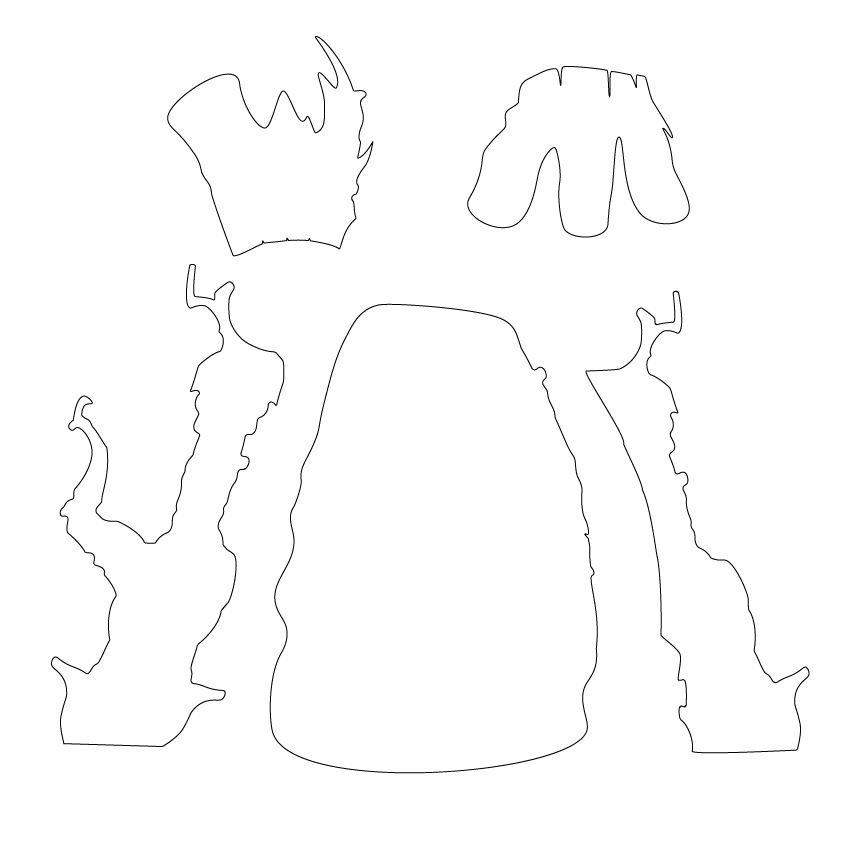
\includegraphics[width=0.4\textwidth]{img/Art/Ent.png}
            \caption{Line art}
            \label{fig:lineart}
        \end{center}
        
        \columnbreak
        
        \begin{center}
            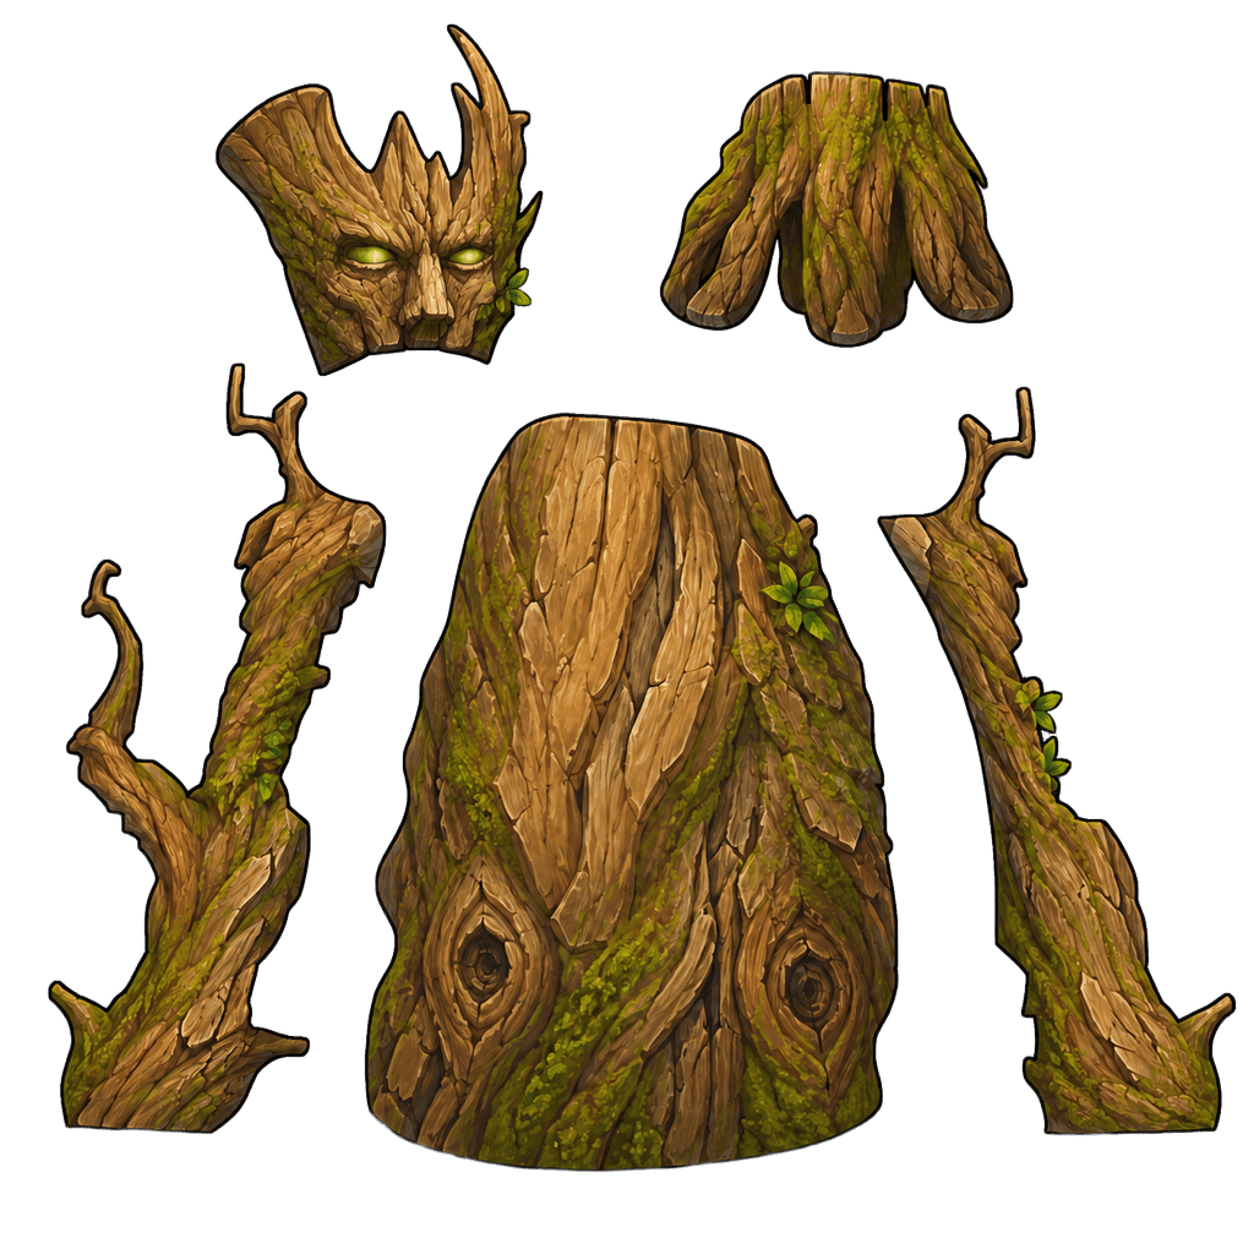
\includegraphics[width=0.4\textwidth]{img/Art/Texturizado GPT.png}
            \caption{AI Texturing}
            \label{fig:texturing}
        \end{center}
    \end{multicols} % Fin de las dos columnas
\end{figure}

The missions also required specific visual resources. Some assets were created or adapted for the project, and others were selected from external asset libraries such as the Unity Asset Store and Itch.io, like the dialogue box or the background texture (see Figure \ref{fig:dialoguebox} and \ref{fig:uiboard} ). In the Garden of Hearing mission, the images used as visual clues were processed with filters so that they did not reveal the answer too directly.

\begin{figure}[h]
    \begin{multicols}{2} % Inicio de las dos columnas
        \begin{center}
            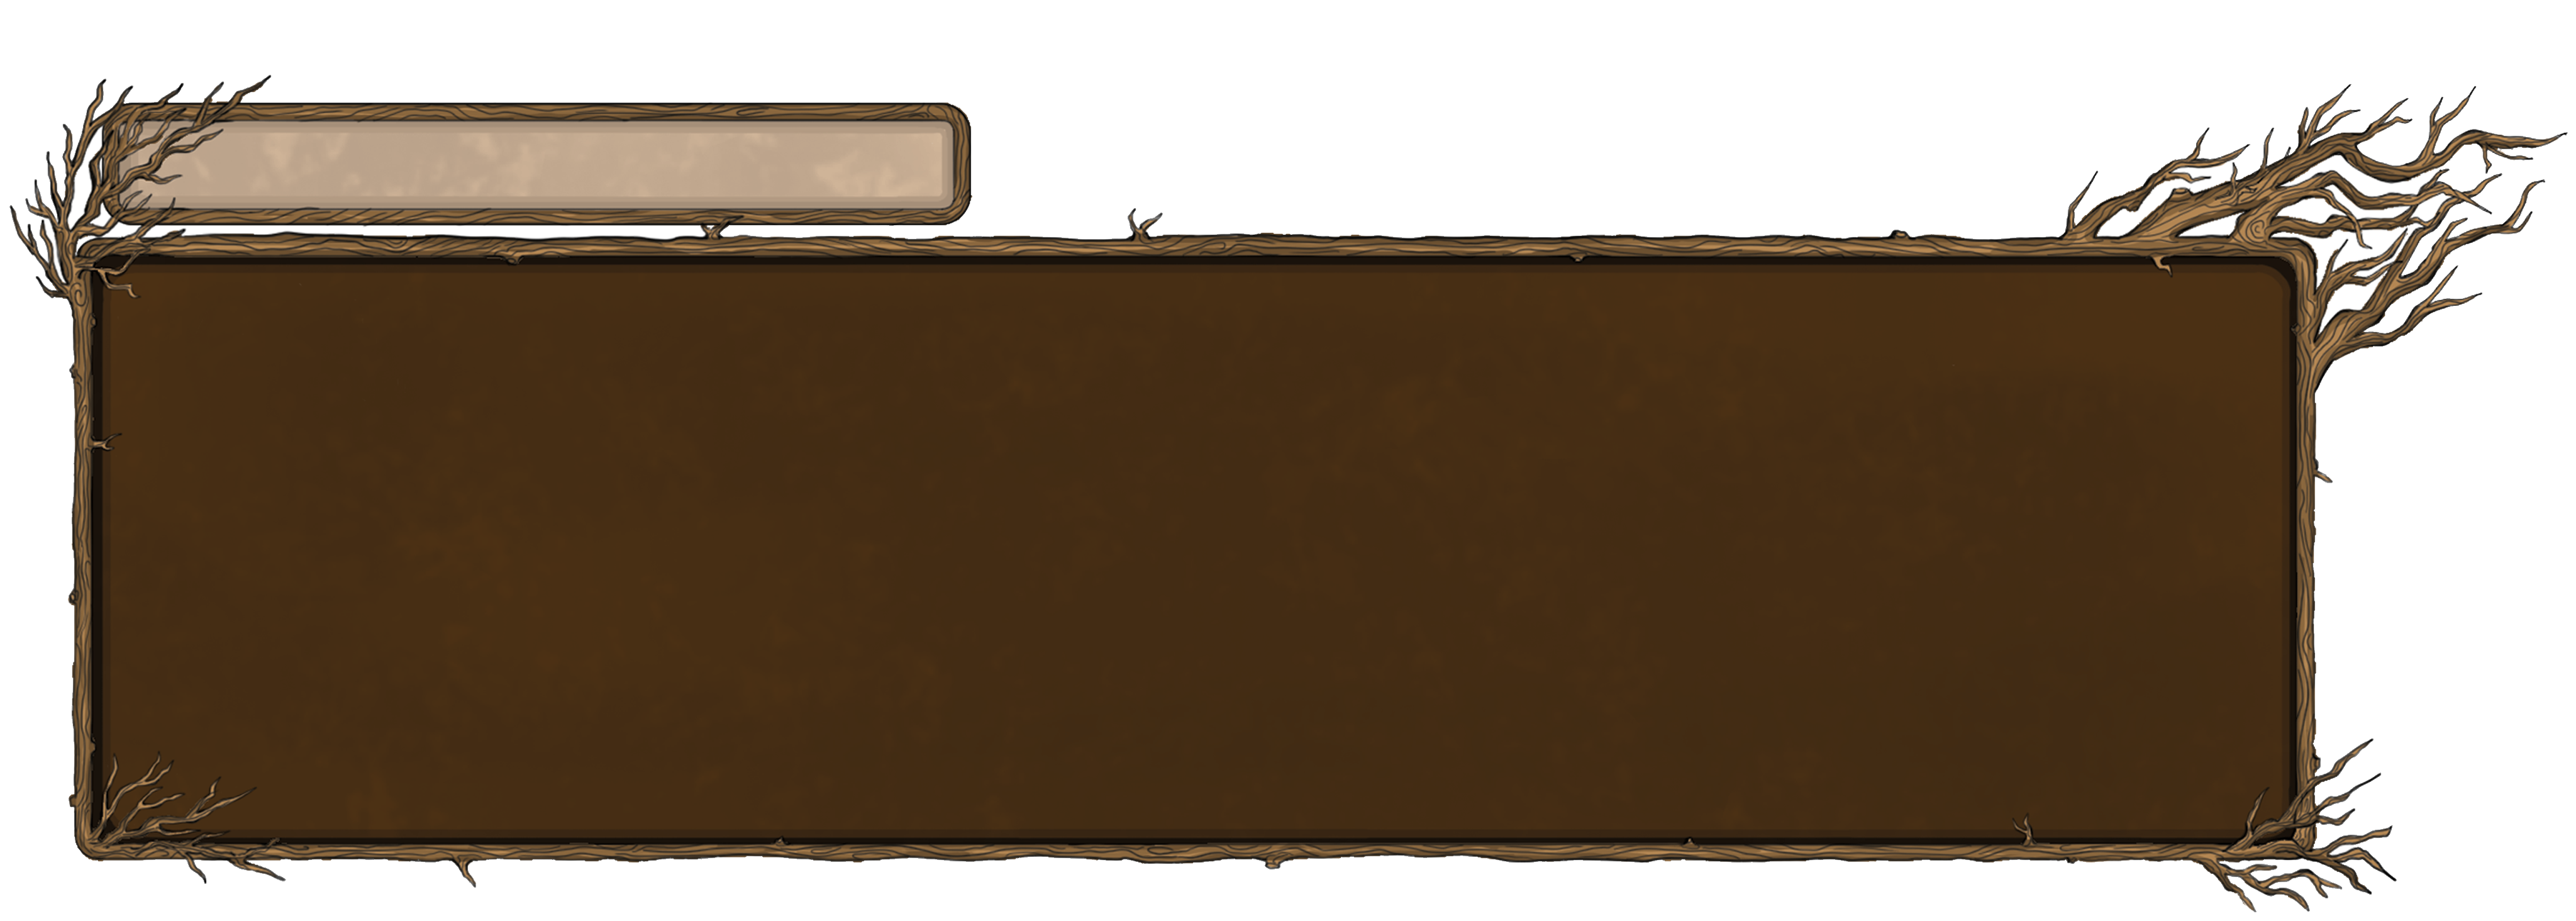
\includegraphics[width=0.4\textwidth]{img/Art/CajaDialogo.png}
            \caption{Dialogue box}
            \label{fig:dialoguebox}
        \end{center}
        
        \columnbreak
        
        \begin{center}
            
\includegraphics[width=0.4\textwidth]{img/Art/UIboard.png}
            \caption{UI board}
            \label{fig:uiboard}
        \end{center}
    \end{multicols} % Fin de las dos columnas
\end{figure}

Audio resources were also part of the artistic and sensory design of the game. Since the Garden of Hearing mission is based on recognising sounds related to the natural environment, sound selection was especially important. For this purpose, specialised sound databases such as Xeno-canto \cite{xenocanto} were used to search for accurate recordings. The selected sounds were recorded in Spain, which helped to keep the audio material coherent with the geographical and environmental context of the project.

In the Testing and Validation section \ref{sec:second_evaluation_cycle}, it will be noted that a way was needed to identify the areas of the garden. Thanks to Águeda, this pair of assets were designed to emulate mycorrhizae: the brown one (Figure \ref{fig:micorrizaMarron}) for when the network is still damaged, and the green one (Figure \ref{fig:micorrizaVerde}) for when the adventurers have repaired the network.
The \textit{Micorrizas} logo shown in Figure \ref{fig:logo} was designed by  Luis to reinforce the visual identity of the game and to make the project easily recognisable.
\begin{figure}[htpb]
    \centering
    
\includegraphics[width=0.2\textwidth]{img/Art/Logo.jpg}
    \caption{The \textit{Micorrizas} logo}
    \label{fig:logo}
\end{figure}
\begin{figure}[h]
    \begin{multicols}{2} % Inicio de las dos columnas
        \begin{center}
            
\includegraphics[width=0.2\textwidth]{img/Art/MicorrizaMarron.png}
            \caption{Mycorrhizal network icon}
            \label{fig:micorrizaMarron}
        \end{center}
        
        \columnbreak
        
        \begin{center}
            
\includegraphics[width=0.2\textwidth]{img/Art/MicorrizaVerde.png}
            \caption{Repaired network area icon}
            \label{fig:micorrizaVerde}
        \end{center}
    \end{multicols} % Fin de las dos columnas
\end{figure}
\newpage
\section{Tecnical Architecture}
The project’s architecture is organised into four main layers: connection and cooperative session, geolocation, spatial representation in ArcGIS, and the cooperative mission layer. Each block has a specific responsibility and communicates with the others via events, synchronised state structures and scene transitions, as can be seen in Figure \ref{fig:architecture}. Appendix \ref{sec:detailed-technical-architecture} provides a much more detailed and technical explanation of this matter.


Firstly, there is a connection and session layer, responsible for launching the application and enabling players to create a co-operative session or join an existing one. This layer establishes the connection between devices before the game begins.

Above this lies the session layer, which maintains the game’s shared global state. In other words, this layer ensures that all players are working with the same information: which mission is active, what stage the game is at, or which elements have been completed.

The geolocation layer retrieves the device’s actual position via GPS and converts it into information useful for the game. In this way, the player’s physical location can be synchronised with the other participants and utilised within the co-operative experience.


Next, the map and spatial representation layer transforms the geographical coordinates into visible and interactive elements within the game, such as markers, trigger zones or points of interest. Thanks to this layer, the real-world space of the \textit{Jardín de los Sentidos} becomes part of the playable world.

Finally, the mission layer organises the game’s activities. This layer is built on a common foundation that allows the general flow of missions to be reused, their results to be managed, and the transition between their different phases to be controlled.
\begin{landscape}
\begin{figure}[p]
    \centering
    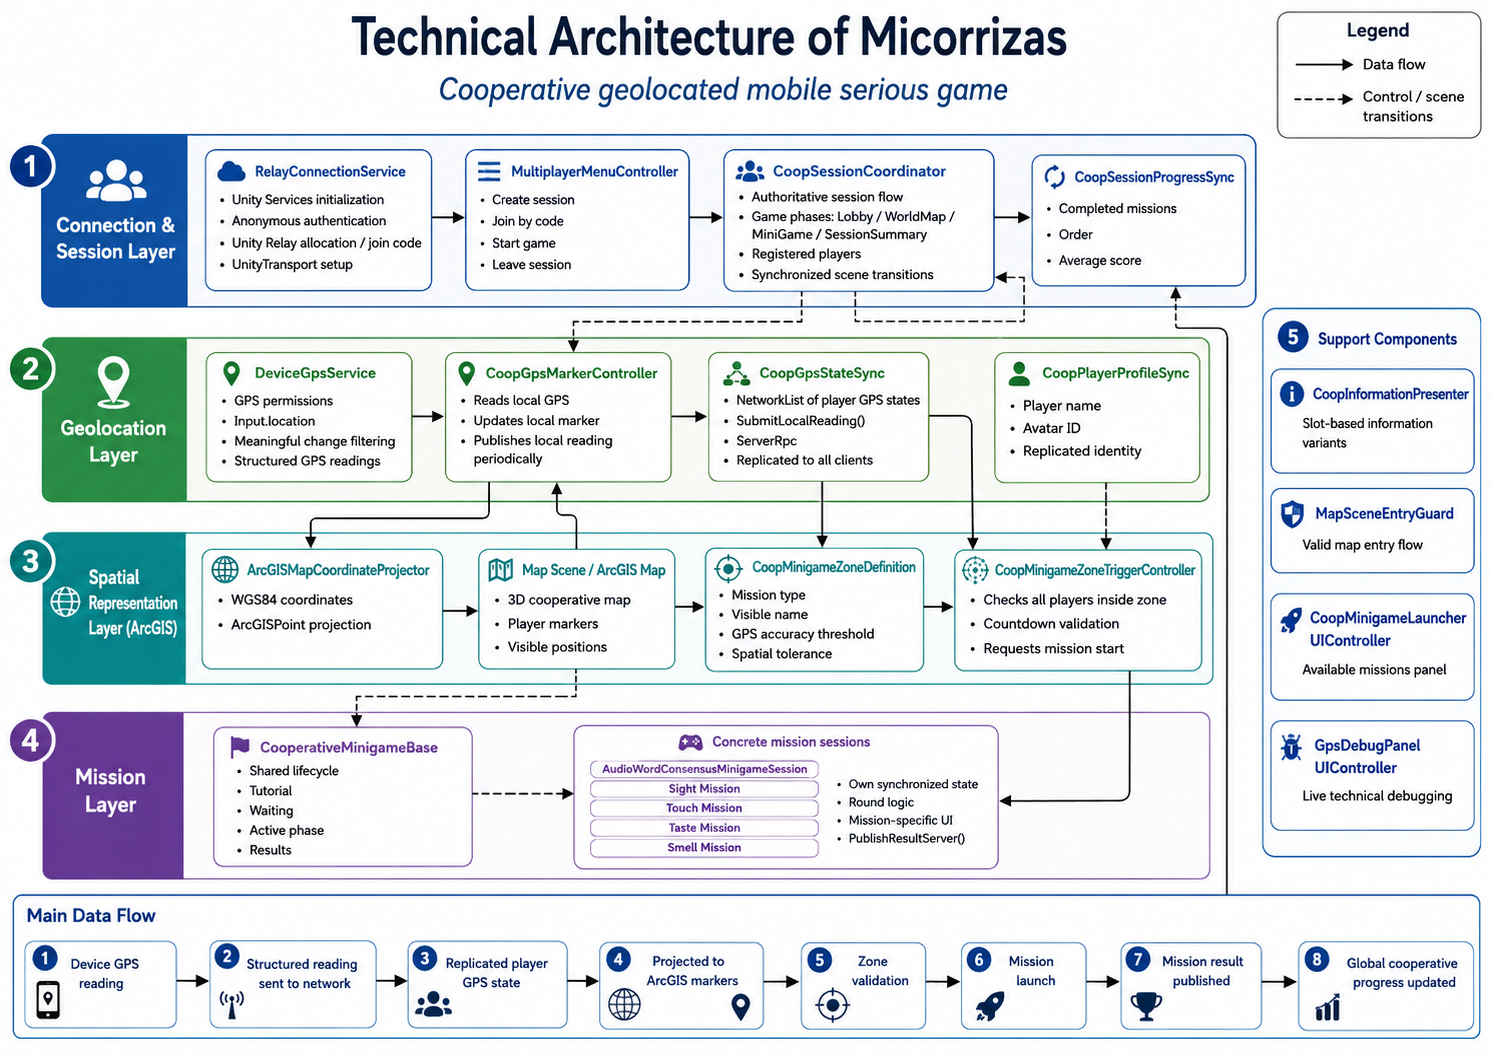
\includegraphics[
        width=\linewidth,
        height=0.85\textheight,
        keepaspectratio
    ]{img/Architecture.png}
    \caption{Micorrizas Architecture}
    \label{fig:architecture}
\end{figure}
\end{landscape}
On a practical level, this architecture relies on tools such as Unity Relay, to facilitate connections between players; Netcode for GameObjects (they are Unity entities, which you can copy and modify), to synchronise information between devices; and the ArcGIS Maps SDK, to work with maps and geographical coordinates. In addition, proprietary services and drivers have been developed to clearly separate data collection, synchronisation, visual representation and the user interface.

The overall architecture begins with the connection and session layer (Point 1 in Figure \ref{fig:architecture}), where the game initialises Unity Services, creates a co-op session via Unity Relay, or allows players to join a game using a code. Once the session has been created, the system maintains the game’s global state, the game stages, the connected players and shared progress.
Next comes the geolocation layer (Point 2 in Figure \ref{fig:architecture}), which retrieves the GPS position of each mobile device. This position is filtered, structured and sent to the network so that all players can view the group’s location status in a synchronised manner.

The spatial layer (Point 3 in Figure \ref{fig:architecture}), using ArcGIS, transforms these real-world coordinates into positions within the game map. Thanks to this layer, the Garden of the Senses is represented by markers, mission zones and activation areas that can be used within the experience.

When all players are within a valid zone, the system launches the corresponding quest. The mission layer (Point 4 in Figure \ref{fig:architecture}) manages the common workflow for each activity: tutorial, waiting period, active phase and results. Each specific quest reuses this framework, whilst maintaining its own logic and interface.

Finally, upon completing a mission, the result is published in the co-op session (Point 1 in Figure \ref{fig:architecture}) and the group’s overall progress is updated. Thus, the entire workflow ranges from the device’s GPS reading to spatial validation, the triggering of the quest and the synchronisation of the shared result.

\section{Problems and solutions}
During development, the main difficulties were related to geolocation, mobile testing and the integration of several technical systems into a single gameplay flow.

One technical issue appeared at the beginning of the project because the initial ArcGIS SDK project was created using Unity HDRP. This pipeline was not suitable for the target platform, as HDRP is not compatible with Android builds in the same way as Unity URP. For this reason, the project had to be migrated from HDRP to URP before continuing development. This migration was necessary to make the application compatible with Android devices and to ensure that the final prototype could be tested in the intended mobile environment.

The first major challenge was the implementation and testing of geolocation. As the game relies on the player’s position in a real-world outdoor environment, the system could not be fully validated within the Unity editor. The location service had to be tested on a real Android device, which slowed down the process and made it less predictable. To address this issue, the geolocation system was developed incrementally: first by loading and centring the map, then by limiting the rendered area, and finally by adding trigger zones for each sensory garden. The trigger zones were designed with generous radii to compensate for GPS inaccuracies.

The multiplayer system also required several design and technical decisions. The project required cross-device cooperation, but the gameplay did not require real-time character movement or complex online interaction. For this reason, the multiplayer implementation was limited to session creation, access codes, player connection, synchronisation of shared states, and group scoring. This reduced the system’s complexity whilst preserving the game’s cooperative structure.

Unity Relay also presented connectivity problems when tested on the university Wi-Fi network. The exact cause could not be identified, although it may have been related to network restrictions or blocked ports. For this reason, multiplayer validation was carried out using alternative connections, such as mobile data or other Wi-Fi networks.

A final challenge was integrating the quests with the rest of the application. Each mission had its own interaction model, but they all had to share the same session structure, scoring logic and progression system, so that it could be reused. To resolve this, the quests were connected to a common flow: activation from the map, execution of the challenge, calculation of the group score and return to the main progression.

\section{Deviations from the initial proposal}
The initial proposal was based on creating an escape room or gymkhana inspired by the activity suggested by the Early Childhood Education teachers. This first approach aimed to transform the guided visit into a sequence of challenges distributed throughout the \textit{Jardín de los Sentidos}, using the physical space as the basis for the player’s progression.

After an initial brainstorming process with the project supervisor, the escape room structure was reconsidered. The project started to move towards a mixed reality experience in which users could learn about the biodiversity of the garden through digital information layered over the physical environment. This direction was interesting from a design perspective, since it allowed the real garden to remain central while adding interactive digital content connected to its plants, sensory areas and educational value.

However, after discussing the proposal with the Early Childhood Education teachers, the mixed reality approach was identified as difficult to apply in a realistic educational context. The main limitation was the accessibility of the required technology. A mixed reality experience would depend on specific devices that are not commonly available to students or teachers, making it harder to use the project as a practical tool during the real activity.

For this reason, the project was refocused on mobile devices, whilst ensuring that the main focus of the project remained the biodiversity of the \textit{Jardín de los Sentidos}. This decision made the game more accessible and better suited for use directly in the garden, given that most potential users already own a mobile phone. The mobile platform allowed the project to maintain a connection with the physical space and reducing the technological barriers to the experience. From that point onwards, the design focused on developing a game for Android mobiles that could combine geolocation, cooperative interaction and educational quests within the \textit{Jardín de los Sentidos}.

